%\chapter{models}\label{sec:models}
\section{Numerical Methods}\label{sec:models}

We set up a suite of 15 controlled N-body simulations using the public available code
\verb+Gadget2+. We have three models for the Milky Way and five models
for the Large Magellanic Cloud, the detailed parameters of the models
are resumed in table \ref{tab:MW} and \ref{tab:LMC}. In section
\ref{sec:MW} and \ref{sec:LMC} we discuss the motivation and
observational evidence for these models. The initial conditions of the
Milky Way and the Large Magellanic Cloud model were set up using the
public available code \verb+GalIC+.

In order to reproduce the actual position and velocity of the Large
Magellanic Cloud with respect to the Milky Way in a first infall
scenario, we integrate the orbits backwards analytically from
the present position and velocity.



\subsection{Milky Way models:}\label{sec:MW}

Many groups have attempted to measure the mass of the Milky Way with
different approaches. \verb+Sohn et al 13+ measures the galactocentric
velocity of the Leo I satellite which is moving at $196.0 \pm 19.4
km/s$. This suggest a minimum mass of $M_{vir} =0.75 \times
10^{12}M_{\odot}$. \citep{vandermarel12} using the timing argument
estimate that the mass of the Local Group is $3.17\pm 0.5 \times 10^
{12}M_{\odot}$ this implies that at most the mass of the Milky Way is
$M_{vir} = 2 \times 10^{12}M_{\odot}$. Due to this uncertainty we
model the Milky Way mass within a range of $1-2 \times
^{10}M_{\odot}$.

Following \citep{Gomez15} each of the models of the Milky Way have
a halo, a disk, and a bulge component. The halo is modeled using a
Hernquist profile with the condition that the enclosed mass
within $r_{vir}$ is the same as with an NFW profile see \ref{fig:MW},
for a detailed calculation see \ref{sec:Appendix} and the appendix
in \citep{Vandermarel12}. The concentration of the halo is
computed following \citep{Klypin11} which derives a concentration
mass relation for halos in a $\Lambda CDM$
Universe. Nevertheless, with such a concentration, the disk
have to be more massive in order to reproduce the
observed rotation curve of the Milky Way, or the concentration
parameter should be $\sim 30\%$ larger. Finally, the Disk of the
Milky Way is modeled using an exponential profile disk and
the Bulge with a Hernquist profile, the detailed parameters are
summarized in table \ref{tab:MWmodels}.

\begin{table}[H]{\label{tab:MW}}
\begin{center}
\begin{tabular}{c c c c c c c c c c c c}
\hline
\hline
$M_{vir} $ & $R_{vir}$ & $r_s$ & $M_{disk}$ & 10 & $M_{bulge}$ & $c_{bulge} $ & $M_{Halo}$ & $c_{halo}$ & $R_{vir, halo}$ & $M_{H,halo}$ & $r_h $ \\
\hline
100 & 261 & 26.47 & 6.5 & 3.5 & 1.0 & 0.7 & 92.5 & 9.918 & 255.82 & 135 & 53.73 \\
150 & 299 & 31.27 & 5.5 & 3.5 & 1.0 & 0.7 & 143.5 & 9.59 & 294.6 & 211  & 61.3 \\
200 & 329 & 35.15 & 5.0 & 3.5 & 1.0 & 0.7 & 194 & 9.38 & 325.8 & 289 & 69.2 \\
\hline
\end{tabular}
\caption{Summary of the Milky Way models \& parameters.\label{tab:MWmodels}}
\end{center}
\end{table}

%The concentration parameter was derived using the relation from 
%\verb+\citep{klypin11}+

%\begin{equation}
%c(M_{vir}) = 9.6(\dfrac{Mvir}{10^12 h^{-1} M\odot})^{-0.075}
%\end{equation}

%$c(1E12) = 9.86$, $c(1.5E12) = 9.99$, $c(2E12) = 10.12$. 

%And the $R_{vir}$ is derived from:

%\begin{equation}
%R_{vir} = \left( \dfrac{2 G M_{vir} }{\Delta_{vir} \Omega_m H^2 } \right)^{1/3}
%\end{equation}

%The constants are $H = H_0 = 3.2407789E-18 h/s$ (this value of H is taken 
%from GalIC) where $h=0.7$. $\Omega_m = 0.27$ and $\Delta_{vir}=360$ at $z=0$. 

%\begin{figure}[H]
%\centering
%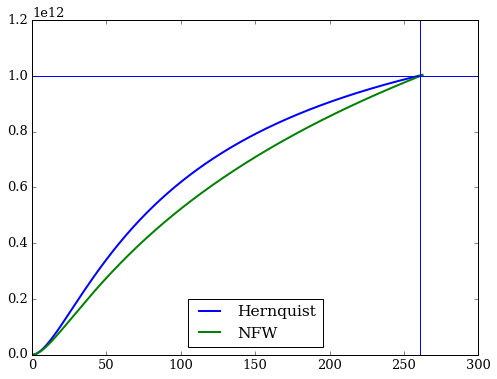
\includegraphics[scale=0.4]{MW_enclosedM.png}
%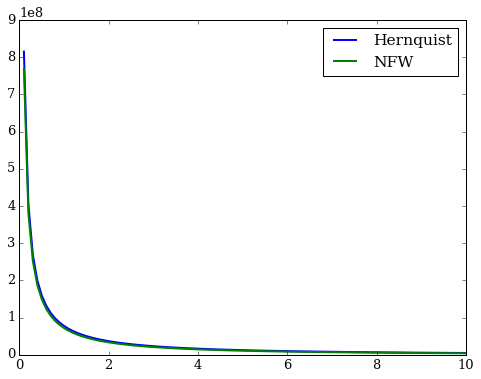
\includegraphics[scale=0.4]{MW_enclosedRho.png}
%\end{figure}

%The initial conditions that are the input values in the GalIC code are:


%This values comes from the code \verb+GalIC_input.py+ the code needs 
%as parameter $Rvir$ and $r_s$ and it runs as follows:

%\begin{verbatim}
%python GalIC_input.py 9.25E11 255.8275 25.79402
%\end{verbatim}

%The IC corresponds to the ouput of $V_{vir}$ and $CC$, GalIC was modified 
%in order to derive the Hernquist equivalence mass and the scale length for a
%Hernquist profile.

%-------------------------------------------------------------------------------

\subsection{Large Magellanic Cloud models:}\label{sec:LMC}

The mass of the LMC is also uncertain, the rotation curve peaks at
$v_c = 91.7 \pm 18.8 km/s$ \citep{vandermarel14} and remains flat
up to $8.7 kpc$, this set a mass of $M(8.7 kpc) = 1.7 \pm 1 \times 10^{10} M_{\odot}$.
There is also evidence that the LMC extends up to $15 kpc$ which in
this case set the minimum value of the LMC at $3 \times 10^{10}
M_{\odot}$. However due to the interaction with the Milky Way dark
matter halo the Large Magellanic cloud have loss material. \verb+\citep{Fox
14}+ have estimated that the mass outside the Large Magellanic Cloud
at $55 kpc$ is $2\times 10^{9} M_{\odot}$, nevertheless, the Magellanic
stream has been observed up to $100 kpc$ which could increase the
baryonic mass up to $4\times 10^{9} M_{\odot}$. Using baryon fraction
arguments the maximum mass of the Large Magellanic Cloud at infall is
$1.7 \times 10^{11} M_{\odot}$.

We use a Hernquist profile to model the dark matter halo of the
Large Magellanic Cloud. The model mass and parameters are resumed 
in table \ref{tab:LMC}.
The scale length was derived in such a way that the enclosed
mass $M(9kpc) = 1.3 \times 10^{10} M_{\odot}$ see Figure XX. The
corresponding rotation curves of these models are shown in Fig XX.



\begin{table}[H]{\label{tab:LMC}}
\begin{center}
\begin{tabular}{c c c c c c c}
\hline
\hline
$M_{LMC} (10^10M\odot)$ & 3 & 5 & 8 & 10 & 18 & 25 \\
$r_p(kpc)$ & 8 & 11 & 14 & 15 & 20 & 22.5 \\
$r_h(kpc)$ & 4.91 & 8.97 & 13.75 & 16.43 & 25.13 & 30 \\
$r_h(kpc)$ & 3.13 & 6.64 & 10.81 & 13.13 & 20.7 & 26.02 \\
\hline
\end{tabular}
\end{center}
\caption{Large Magellanic Clouds parameters \label{tab:LMC}}
\end{table}
%---------------------------Plummer--------------------

%The enclosed mass for the Plummer profile is shown in Fig.\ref{fig:LMC_mass_p}.


%\begin{figure}[H]{\label{fig:LMC_mass_p}}
%\centering
%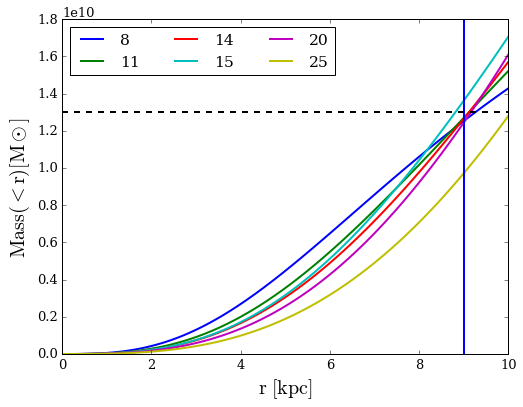
\includegraphics[scale=0.4]{LMC_mass_plummer.png}
%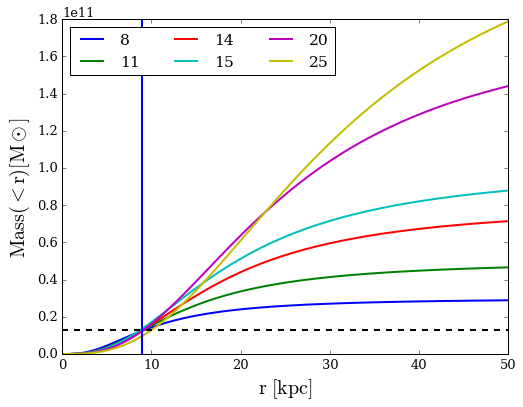
\includegraphics[scale=0.4]{LMC_mass_plummer_out.png}
%\end{figure}
%While the rotation curve is shown in \ref{fig:LMC_rotcurve_p}. \\
 
%\begin{figure}[H]{\label{fig:LMC_rotcurve_p}}
%\centering
%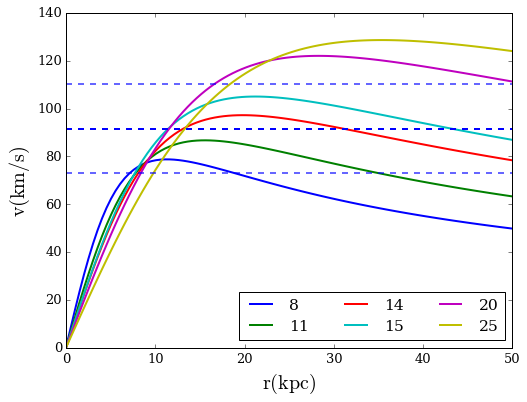
\includegraphics[scale=0.4]{LMC_rotcurve_plummer.png}
%\end{figure}



%---------------------------Hernquist------------------


%The enclosed mass for the Hernquist profile is shown in Fig.\ref{fig:LMC_mass}.

%\begin{figure}[H]{\label{fig:LMC_mass}}
%\centering
%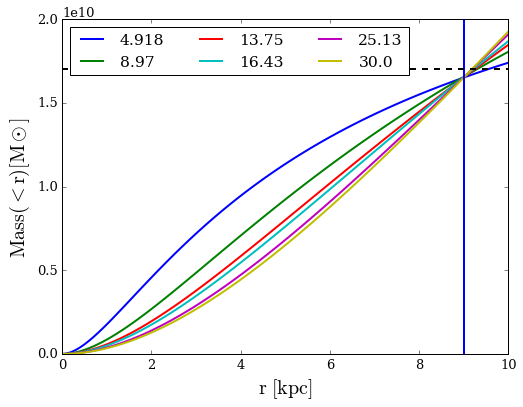
\includegraphics[scale=0.4]{LMC_mass_hernquist.png}
%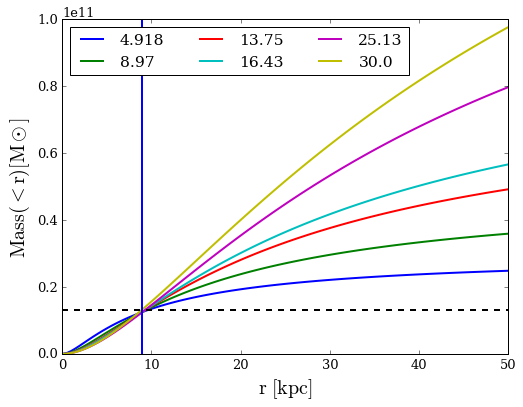
\includegraphics[scale=0.4]{LMC_mass_hernquist_out.png}
%\end{figure}

%While the rotation curve is shown in \ref{fig:LMC_rotcurve}.

%\begin{figure}[H]{\label{fig:LMC_rotcurve}}
%\centering
%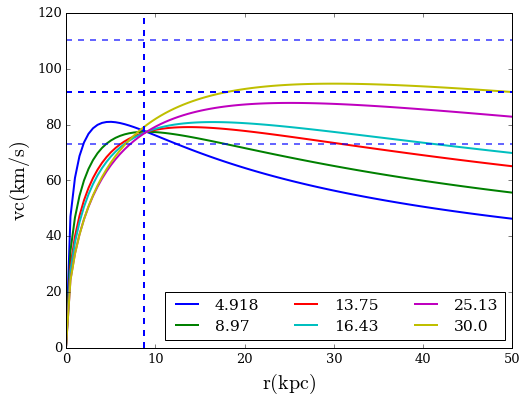
\includegraphics[scale=0.4]{LMC_rotcurve_hernquist.png}
%\end{figure}


%The enclosed mass for the Hernquist profile is shown in Fig.\ref{fig:LMC_mass}.

%\begin{figure}[H]{\label{fig:LMC_mass}}
%\centering
%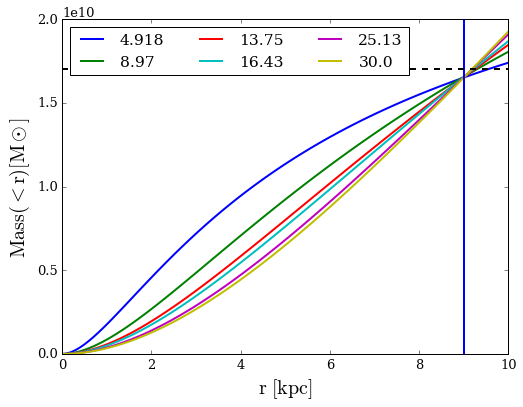
\includegraphics[scale=0.4]{LMC_mass_hernquist_2.png}
%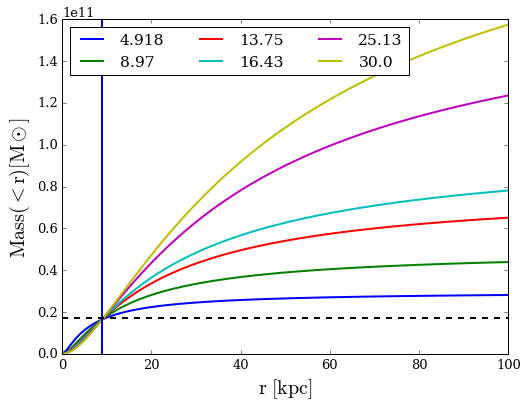
\includegraphics[scale=0.4]{LMC_mass_hernquist_out_2.png}
%\end{figure}

%While the rotation curve is shown in \ref{fig:LMC_rotcurve}.

%\begin{figure}[H]{\label{fig:LMC_rotcurve}}
%\centering
%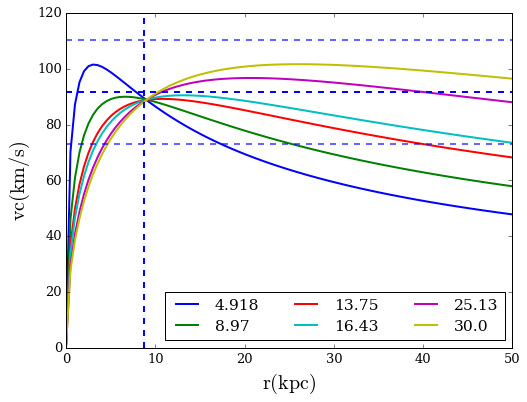
\includegraphics[scale=0.4]{LMC_rotcurve_hernquist_2.png}
%\end{figure}

%\subsection{GalIC modification}

%In order to compute the Hernquist scale length $a$ and the Hernquist equivalent mass 
%the code do the following:

%\textbf{Input parameters:} CC (Halo Concentration Parameter of the NFW profile) and Vvir (Virial Velocity of the NFW halo km/s).\\
%In our case this values are $M_{vir} = 1E12 M\odot$ and $CC = c_{vir} = 9.86$ \\
%With these parameters we compute the \textbf{output parameters:} $M_H$ (Virial mass of the equivalent Hernquist profile) and $a$.

%using:

%\begin{equation}
%M_{vir} = \dfrac{V_{vir}^3}{\sqrt(48.6) H G}
%\end{equation}

%\begin{equation}
%R_{vir} = \dfrac{V_{vir}}{\sqrt(48.6)H}
%\end{equation}

%In the code $H = 3.2407789E-18 h / s$. \\

%Which leads to $M_{vir} =  7E11 M\odot / h $ and $R_{vir} = 183.67 Kpc / h  = 262.38 kpc$ \\
 
%With $R_{vir}$ and $c_{vir}$ $r_s$  could be derived: \\

%\begin{equation}
%r_s = \dfrac{R_{vir}} {c_{vir}} = 18.62 kpc/ h = 26.6 kpc
%\end{equation} 

%To get the Equivalent Hernquist mass we first we have to get the ratio $a$

%\begin{equation}
%a = \dfrac{r_s}{(2 f(c_{vir}))^{-1/2} - 1/c_{vir}} = 38.77 kpc/ h  = 55.38 kpc
%\end{equation}

%Where $f(c_{vir}) = ln(1 + c_{vir}) - c_{vir}/(1+c_{vir})$

%Finally the Hernquist Mass is computed with:

%\begin{equation}
%M_H = \dfrac{M_{vir} (a/r_s)^2}{2f(c_{vir})} = 1.02E12 M\odot / h = 1.45E12 M\odot
%\end{equation}

%\subsection{Analytic:}

%For the analytic we derive $M_H$ using the same procedure explained above and we get: \\

%$M_H = 1.46E12 M\odot$ and  $a = 53.06 kpc$. 

%Where we start from $Rvir = 261 kpc$, $r_s = 26.47$ and $M_{vir} = 1E12 M\odot$

